%%
%% This is file `sample-sigplan.tex',
%% generated with the docstrip utility.
%%
%% The original source files were:
%%
%% samples.dtx  (with options: `sigplan')
%% 
%% IMPORTANT NOTICE:
%% 
%% For the copyright see the source file.
%% 
%% Any modified versions of this file must be renamed
%% with new filenames distinct from sample-sigplan.tex.
%% 
%% For distribution of the original source see the terms
%% for copying and modification in the file samples.dtx.
%% 
%% This generated file may be distributed as long as the
%% original source files, as listed above, are part of the
%% same distribution. (The sources need not necessarily be
%% in the same archive or directory.)
%%
%% The first command in your LaTeX source must be the \documentclass command.
\DocumentMetadata{
  lang=en,
  pdfversion=2.0,
  %pdfstandard=ua-2,
  %testphase={phase-III,firstaid,math,title}
  tagging=on,
  testphase={phase-III,firstaid,math,title}
  %tagging-setup={math/setup=mathml-SE}
}
\documentclass[sigplan,screen,nonacm]{acmart-tagged}
\usepackage{color}
\setlength {\marginparwidth }{2cm}
\usepackage[colorinlistoftodos]{todonotes}
\usepackage[
    type={CC},
    modifier={by-nc-sa},
    version={4.0},
]{doclicense}
%% NOTE that a single column version is required for 
%% submission and peer review. This can be done by changing
%% the \doucmentclass[...]{acmart} in this template to 
%% \documentclass[manuscript,screen,review]{acmart}
%% 
%% To ensure 100% compatibility, please check the white list of
%% approved LaTeX packages to be used with the Master Article Template at
%% https://www.acm.org/publications/taps/whitelist-of-latex-packages 
%% before creating your document. The white list page provides 
%% information on how to submit additional LaTeX packages for 
%% review and adoption.
%% Fonts used in the template cannot be substituted; margin 
%% adjustments are not allowed.
%%
%% \BibTeX command to typeset BibTeX logo in the docs
\AtBeginDocument{%
  \providecommand\BibTeX{{%
    \normalfont B\kern-0.5em{\scshape i\kern-0.25em b}\kern-0.8em\TeX}}}


%%
%% end of the preamble, start of the body of the document source.
\begin{document}

\title{Challenges of Optical Character Recognition}
\author{Orville ``El'' Anderson}
\email{and10393@umn.edu}
\affiliation{
  \institution{Division of Science and Mathematics 
	\\
        University of Minnesota, Morris
	}
  \city{Morris}
  \state{Minnesota}
  \country{USA}
  \postcode{56267}
}

%%
%% The abstract is a short summary of the work to be presented in the
%% article.
\begin{abstract}
Optical Character Recognition (OCR) is technology used to extract text from images. OCR has three main weaknesses when applied to scanned documents stemming from page layouts, the alphabet used, and visual noise. By intentionally expanding the documents we use to train modern OCR models, we can increase [usability] of this technology. This paper looks at the Tesseract, Amazon Textract, and Google Document AI models, as applied to English and Arabic documents.
\end{abstract}

\doclicenseThis

%%
%% Keywords. The author(s) should pick words that accurately describe
%% the work being presented. Separate the keywords with commas.
\keywords{optical character recognition, scanned documents, layout, languages, visual noise, datasets}


%%
%% This command processes the author and affiliation and title
%% information and builds the first part of the formatted document.
\maketitle

\section{Introduction}
\label{sec:introduction}

There is a wide variety of documents that have been photographed\footnote{passive voice...}. These images are popular because they are easy to create and share. These images are inferior to traditional digital documents in the sense that they [are not search-able] or editable without fundamentally changing the structure.\footnote{garbage} Optical Character Recognition is a [technology] made to extract text from images. This paper looks at how OCR works, specifically for scanned documents, and looks at some of the specific weaknesses in applying OCR to these documents.

\section{Background}
\label{sec:background}

The first step in using OCR on a document is to acquire an image of the document. This can be done using a camera or a scanner. These images can be saved as a variety of formats, such as a .pdf, .jpg, or .png. This file is then input to an OCR model, such as Tesseract, Textract, or Document AI\footnote{Document AI can mean many things, even within the topic of OCR, here in this paper it specifically means the OCR model Google Document AI} where the model will go through the three stages of OCR. The model will then return the text identified in the document as plain text.\footnote{There are some models which also return information about where they found each character and with this they can output the text in a variety of formats.} 
%There exists variations in models, where some will also output information about where in the image a character was found. The text identified and the optional [information] can be returned in a variety of formats, depending on the model.

Pages to Reference\cite{Raj:2022,Avyodri:2022,Thorat:2022}

\subsection{Document Layout Analysis}
\label{DLA}

The first step in OCR is Document Layout Analysis (DLA), and is a general pre-processing step. The purpose is to identify what part of the image is text and what is not. 
% This step addresses some of the complexity introduced when the image was made. This step can include rotating the full image and cropping out borders.
This step frequently includes converting the input image to a binary image, where each pixel is marked as a text or non-text pixel, to reduce computation costs.

\subsection{Text Line Detection}
\label{TLD}

Text Line Detection (TLD) is the second step in OCR. TLD takes the blocks of text from the previous step and further breaks them down into lines, words, and then characters. The output of this step is each identified character in its own defined box of pixels.

% A common technique used in this step includes rotating the individual lines to create a baseline for each line of text. 
% This step consists of breaking up blocks of text into lines of text, then into individual words, then letters.

% After the individual characters have been identified, we go through and look at each of the boxes we have drawn around the characters and mark which pixels we think are text and which are not.

%\begin{figure}
%  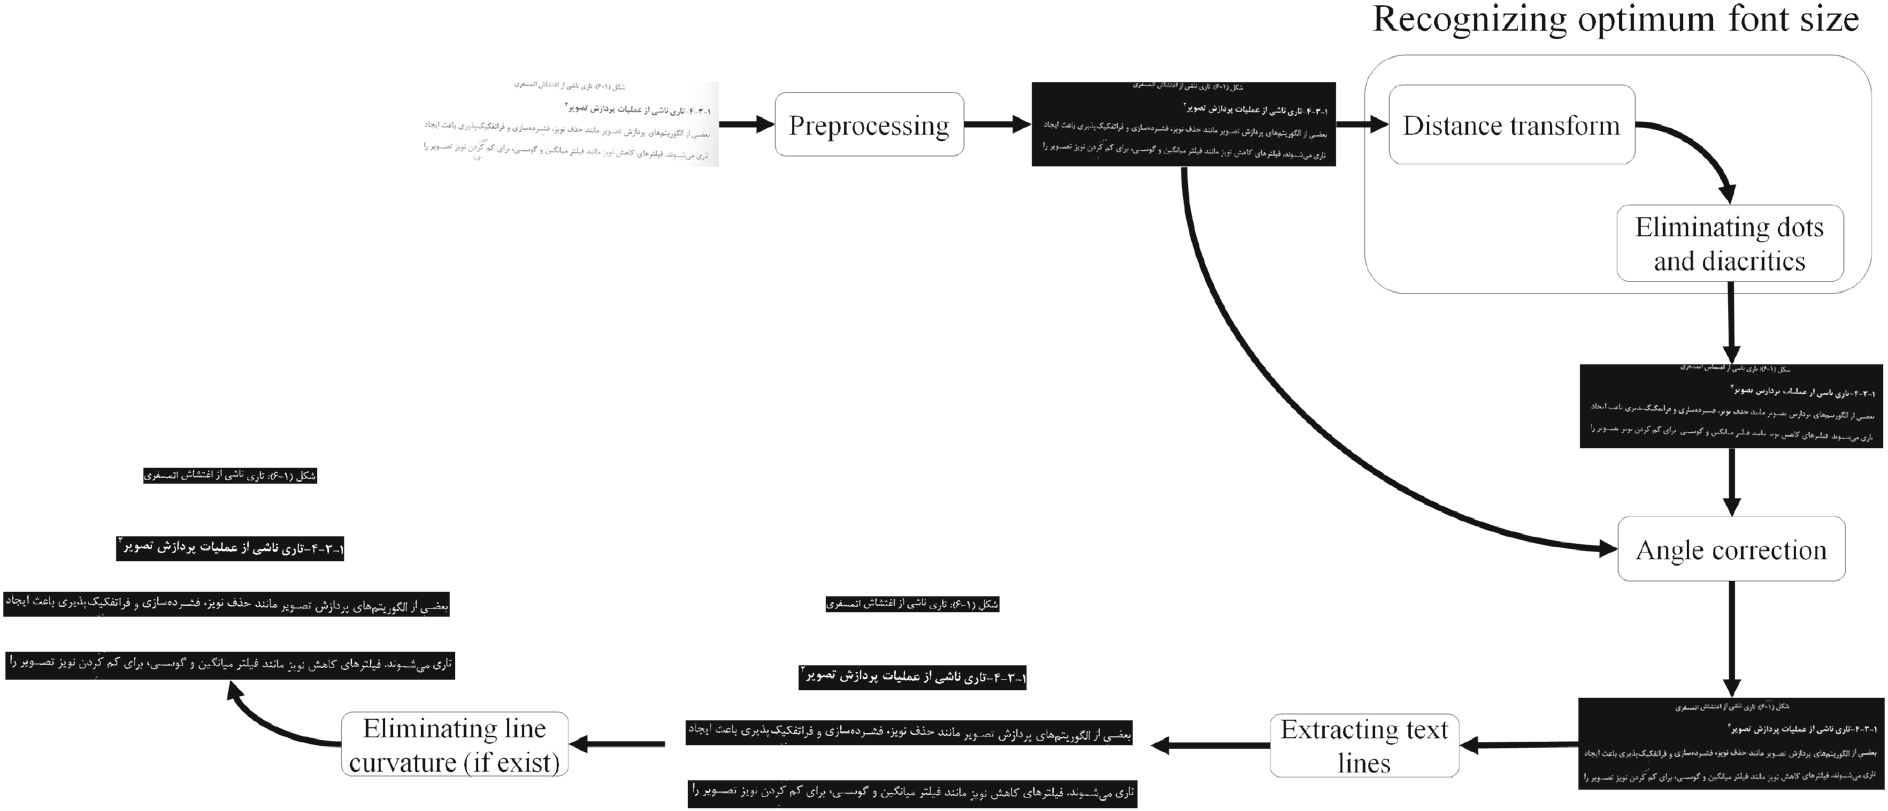
\includegraphics[width=\linewidth]{TLD.png}
%  \caption{stages of TLD}
%  \label{fig:tld}
%\end{figure}

\subsection{Recognition}
\label{Recognition}

The final step in the OCR process is referred to as Classification or Recognition. This step takes the boxes of individual characters from the last step and tries to identify the character inside of them.

One common technique is to compare the unknown character to a set of known characters, overlaying them, and seeing which ones are the most similar. Another technique is to identify features from the character to make an educated guess.\citep{Thorat:2022}\footnote{Objection, how is this relevant?? Wouldn't it be more important to talk about training for recognition?}
%There are many ways to do this, but it boils down to matching your letter to a whole bunch of other letters and seeing which one is closest.
%One very common method for character recognition is to use a Deep Learning. (woo magic). The notable thing about this method is that it must be intentionally fed examples of text to train.

%\subsection{Post-Processing}
%\label{sec:Post-Processing}
%
%Post-processing is an optional, but very common step for OCR, consisting of spellcheck and formatting. Running spellcheck on the output generally improves accuracy, but will write over spellings from the source document(misspellings and unconventional spellings included.) The additional formatting step is used to return the document to a human readable form. Some OCR will place the output directly over the input image, some will make webpages with the output and some will --.

\subsection{Comparison}
\label{comparison}

The main considerations when judging OCR models are accuracy and speed.\cite{Raj:2022} 

%[Speed is measured with a timer]

A popular way to measure the accuracy of OCR output is to run the OCR program on a document where the page content is know. The OCR output is then compared to the known content and is measured by [the formula below], where x is a unit of measurement, like a line, word, or character.
\[
\dfrac{\sum\limits_{i=1}^\text{num of pages}\text{number of x correctly indentified}}{\sum\limits_{i=1}^\text{num of pages}\text{number of x on the page}}
\]

% \cite{Hegghamer:2022} this paper makes a destinction between word accuracy and character accuracy saying that "----"

\section{Challenges}
\label{sec:body}

There are three main categories of things that make scanned documents harder to digitize. Each of these challenges tie back to the key concept that OCR models work best when applied to what they were made to recognize.

\subsection{Layout}
\label{Layout}

Documents come in many different layouts. Things like images, figures, and number of columns add a layer of complexity to documents. 
In the Document Layout Analysis step of OCR the model must know which parts of the page to ignore, but also to know what order the sections of text should go in.
A paper formatted with two columns, such as this, is meant to be read left column, then right column. Unless otherwise instructed, an OCR model will take the first line from each column and treat them as one line. 
% While understanding paragraph breaks and readign order is generally intuitive, this is something that must be intentionally taken into account when training OCR.

There exists OCR specifically trained to handle documents like forms. For example a model can be trained to specifically digitize job applications for a specific company, or one specific tax form. By making a specialized  model, there is an increased accuracy when working with documents of that specific layout, but a decrease in accuracy for other layouts. 

One related challenge to OCR accuracy is curved lines of text. The DLA and TLD stages of OCR\footnote{don't you dare use another acronym in this paragraph} use rectangles to section off portions of text and do not automatically rotates lines/words/characters to be [horizontal?]. Identifying a character when it is rotated is less likely to be accurate then if the character was horizontal. \citep{Fateh:2024}

\subsection{Alphabet}
\label{Alphabet}

The English alphabet consists of 26 letters, each with a lowercase and uppercase variant. English is written left-to-right and is primarily non-cursive.
Arabic, in comparison is unicase, uses contextual forms, is written right-to-left, and is cursive. Arabic also uses diacritics, dots and marks, which can appear above or below the main text and influence the meaning.

These two languages are important when discussing OCR, both because of their popularity, but also because of how different they are. As this paper\cite{Fateh:2024} says about Arabic, "Finally, character and TLD approaches cannot be universally applied to scripts with different languages. This challenge is particularly pronounced in languages such as Persian and Arabic, where text characters can take the form of connectors or non-connectors. Connector letters are affixed to both pre- and post-letters to form words, and diacritic marks are commonly used in Arabic text—both of which can introduce complexity to TLD techniques." This paper explored the effects of changing the size of boxes when isolating characters in Arabic documents. They found that by increasing the size of the boxes, they had a higher accuracy. 

\todo[inline]{I introduce a lot of concepts here (like reading direction) that I don't do anything with. I need to touch on them, or remove them}

% Variations in fonts and alphabets introduce an added layer of complexity that need to be accounted for when performing the character recognition step. 
% In many cases, such as the Cirrilic "", it adds confusion, where the character is mis-classififed as the Latin "H".
% These models are not automatically applicable to other alphabets.  This inherently gives all other languages a bit of a disadvantage. Other alphabets also have nuances that make it harder to directly apply OCR to. A common example is Arabic. (there's dots) \cite{Fateh:2024, Hegghamer:2022}

This weakness in OCR models is most easily seen in non-Latin language documents, but can also be seen when using these models on documents with a variety of fonts, or documents with handwritten text. 

\subsection{Visual Noise}
\label{Noise}

% There's so many ways to scan a document badly. \cite{Hegghamer:2022}
One big factor in the accuracy of OCR is the quality of the initial image. Marks on the physical document, book spines, and low image resolution all add additional complexity to the process. 



\section{Results}
\label{sec:Results}

To evaluate accuracy and compare OCR models we use bench-marking datasets, collections of images where the expected output is known. Because of the inherit variety of documents needed to target these issues there is not really a reasonable way to make one. Some specialized data-sets exist \cite{Fateh:2024,Hegghamer:2022}

Fateh et Al\citep{Fateh:2024} looks at TLD for Arabic text and found that increasing the size of the boxes drawn around each character increased OCR output accuracy(for the model(s) they tested)

Thomas Hegghamer created an English and Arabic dataset specifically to test OCR accuracy of documents with artificial noise applied. "functions to generate six ideal types of image noise: “blur,” “weak ink,” “salt and pepper,” “watermark,” “scribbles,” and “ink stains” (see Fig. 2c-h). While not an exhaustive list of possible noise types, they represent several of the most common ones found in historical document scans."\citep{Hegghamer:2022} Hegghamer's "Noisy OCR Dataset", consists of 422 original documents with 43 variations of each, for a total of 18,568 documents.

\section{Conclusion}
\label{Conclusion}

If the end goal of Optical Character Recognition for documents is to make one model that can be used on all documents to ever exist, it makes sense to have an all-encompassing weakness-addressing data set. As it stands, that data set can not exist. Ignoring the obvious storage and resource considerations, for the reasons outlined in this paper, we can not begin to comprehend the number of variations in documents, let alone truly test for them all. 

A universal data set would not be widely accepted because it would actively go against many popular forms of OCR, specialized layout OCR models. While not generally applicable, due to their specialized nature, these models have a place in OCR conversations.

All that said, I think that ideal data set is worth perusing. Progress towards a goal we may never meet is still progress. By pushing the bounds of what OCR models can do, we can strengthen their current capabilities.

\todo[inline]{dataset or data set?}

%* Its a nice idea to make one data set to address all of these issues
%* That's impossible tho
%* That wouldn't be widely used/accepted (gonna skip this point)
%* It's still worth working towards
%
%
%While it's ideal to have one golden bench-marking set, that's hard (because of the reasons outlined above), so now we have specialized ones. 
%Honestly I don't have a full stance on if I think these specialized sets are good. Yes, they highlight weaknesses of general OCR models, and push the development of OCR further, but blind acceptance and promotion of them can neglect some of the specialties of OCR, like layout-specific models. Data sets also don't really encourage reducing time and resource complexity for models, which I would like to see.
%I am interested in this topic of OCR because of the role I think it could play in digital accessibility, but for that we would need to push for more free models with graphic user interfaces.\footnote{for context, Document AI and Textract are both paid models, and Tesseract only has 3rd party GUIs} 

%% Elena: examples like this are actually helpful, but I can't locate theit bibliography 
%% file (I think they are using a database), so providing examples will have to wait.

%  Some examples.  A paginated journal article \cite{Abril07}, an
%  enumerated journal article \cite{Cohen07}, a reference to an entire
%  issue \cite{JCohen96}, a monograph (whole book) \cite{Kosiur01}, a
%  monograph/whole book in a series (see 2a in spec. document)
%  \cite{Harel79}, a divisible-book such as an anthology or compilation
%  \cite{Editor00} followed by the same example, however we only output
%  the series if the volume number is given \cite{Editor00a} (so
%  Editor00a's series should NOT be present since it has no vol. no.),
%  a chapter in a divisible book \cite{Spector90}, a chapter in a
%  divisible book in a series \cite{Douglass98}, a multi-volume work as
%  book \cite{Knuth97}, a couple of articles in a proceedings (of a
%  conference, symposium, workshop for example) (paginated proceedings
%  article) \cite{Andler79, Hagerup1993}, a proceedings article with
%  all possible elements \cite{Smith10}, an example of an enumerated
%  proceedings article \cite{VanGundy07}, an informally published work
%  \cite{Harel78}, a couple of preprints \cite{Bornmann2019,
%    AnzarootPBM14}, a doctoral dissertation \cite{Clarkson85}, a
%  master's thesis: \cite{anisi03}, an online document / world wide web
%  resource \cite{Thornburg01, Ablamowicz07, Poker06}, a video game
%  (Case 1) \cite{Obama08} and (Case 2) \cite{Novak03} and \cite{Lee05}
%  and (Case 3) a patent \cite{JoeScientist001}, work accepted for
%  publication \cite{rous08}, 'YYYYb'-test for prolific author
%  \cite{SaeediMEJ10} and \cite{SaeediJETC10}. Other cites might
%  contain 'duplicate' DOI and URLs (some SIAM articles)
%  \cite{Kirschmer:2010:AEI:1958016.1958018}. Boris / Barbara Beeton:
%  multi-volume works as books \cite{MR781536} and \cite{MR781537}. A
%  couple of citations with DOIs:
%  \cite{2004:ITE:1009386.1010128,Kirschmer:2010:AEI:1958016.1958018}. Online
%  citations: \cite{TUGInstmem, Thornburg01, CTANacmart}. Artifacts:
%  \cite{R} and \cite{UMassCitations}.


%%
%% The acknowledgments section is defined using the "acks" environment
%% (and NOT an unnumbered section). This ensures the proper
%% identification of the section in the article metadata, and the
%% consistent spelling of the heading.
\begin{acks}
Thanks.
\end{acks}

%%
%% The next two lines define the bibliography style to be used, and
%% the bibliography file.
\bibliographystyle{ACM-Reference-Format}
\bibliography{sample_paper}

\end{document}
\endinput
%%
%% End of file `sample-sigplan.tex'.
